\documentclass[10pt,a4paper]{article}
\usepackage[margin=23mm]{geometry}
\usepackage[T1]{fontenc}
\usepackage{lmodern}
\usepackage{microtype}
\usepackage{booktabs}
\usepackage{graphicx}
\usepackage{xcolor}
\usepackage{hyperref}
\usepackage{url}
\usepackage{array}
\usepackage{float}
\hypersetup{colorlinks=true,linkcolor=blue,urlcolor=blue}
\setlength{\parskip}{.35em}
\setlength{\parindent}{0pt}
\newcommand{\gain}{\textit{N-to-L gain}}
\newcommand{\src}[1]{\textsuperscript{\cite{#1}}}

\begin{document}
\begin{center}
{\Large\bfseries NumStability benchmark: post-hoc ten-task sensitivity report}\par
\vspace{2mm}
{\small 28 September 2026 \quad | \quad Derived from the sealed Pilot 34/35 fifteen-task composite}
\end{center}

\begin{abstract}
After viewing the fifteen-task outcomes, five tasks were selected for removal:
HI21-EQ2.7, P14-SHIFTED-SUM, P14-ALT-SOFTMAX, P14-SHIFTED-LOG, and
P14-SHIFTED-WEIGHTED. No contestant was rerun and no source result was altered.
In the remaining ten, L (Mathlib plus NumStability) used 19.7\% fewer proof-code
lines and 22.5\% less contestant-active time than N (Mathlib only), excluding
the one-time warm scout. Charging that scout once leaves a 19.9\% time gain.
Across realized-reuse scores 1, 2, and 3, the selected cohort's aggregate
time gains are $-9.1\%$, $+19.3\%$, and $+31.1\%$. This is a stronger
\emph{descriptive} pattern than in the complete corpus. It is not an unbiased
or prospective test: both task exclusions and the five prior favorable retained
tasks depend on observed outcomes; the reuse rubric was also annotated after
the outcomes. Among only the five newly screened tasks still included, L is
7.2\% faster but uses 6.4\% more proof lines.\src{primary,metrics,reuse,derived}
\end{abstract}

\section{What changed, and what did not}

This is a subset analysis of the previously published fifteen-task report,
\emph{not} a replacement benchmark. The user named five exclusions after
inspecting their scores and results on 28 September 2026. The selection rule
was not registered before data collection. The original fifteen-task analysis,
its negative results, frozen prompts and packets, candidate hashes, audit
records, and proof artifacts remain intact. The generated JSON records the
exact excluded IDs and input SHA-256 hashes. All fifteen tasks had faithful
statements and zero-hole Lean-accepted proofs in both conditions.\src{primary,metrics,derived}

The two conditions, formalization/proof stages, four-submission limits per
stage, independent off-clock faithfulness audit, full source access, warm L
orientation, three parallel resource-isolated lanes (eight logical CPUs and
24~GiB each), and hardware are unchanged from the primary report. Both
formalizers used GPT-6 Sol/high; auditors used GPT-6 Astra/high. No new measurement was made
here. ``Time'' below is summed contestant-active seconds; it excludes audit
effort and concurrent campaign makespan. Positive gain means L required less
time, fewer net-new tokens, or fewer nonblank proof-code lines.\src{primary,metrics}

\begin{table}[H]
\centering\small
\begin{tabular}{@{}lrrrrrr@{}}\toprule
Cohort & $n$ & N sec & L sec & Time gain & N lines & L lines\\\midrule
All original tasks & 15 & 10,515 & 8,978 & +14.6\% & 4,913 & 4,413\\
Post-hoc selected & 10 & 6,979 & 5,410 & +22.5\% & 3,158 & 2,537\\
Selected prior favorable & 5 & 3,985 & 2,631 & +34.0\% & 1,869 & 1,166\\
Selected newly screened & 5 & 2,994 & 2,779 & +7.2\% & 1,289 & 1,371\\\bottomrule
\end{tabular}
\caption{Summed results from the sealed pairs. Proof-line gains, respectively,
are +10.2\%, +19.7\%, +37.6\%, and $-6.4\%$. ``Prior favorable'' is an
outcome-aware retained stratum, not a randomized group.\cite{metrics,derived}}
\label{tab:cohorts}
\end{table}

\clearpage
\section{The ten selected tasks}

\begin{table}[H]
\centering\small
\begin{tabular}{@{}lrr rr@{}}\toprule
Task & Reuse score & Origin & Time gain (\%) & Proof-line gain (\%)\\\midrule
\texttt{CAST08-FIXED3} & 3/3 & prior & +35.9 & +32.0 \\
\texttt{P14-T1} & 2/3 & new & +24.9 & -12.9 \\
\texttt{HI21-LEM2.2} & 1/3 & new & -47.1 & -25.6 \\
\texttt{CAST08-PROP3.1} & 3/3 & prior & +35.5 & +46.4 \\
\texttt{P14-T2} & 2/3 & new & +14.6 & +5.2 \\
\texttt{RUMP12-THM3.4} & 3/3 & prior & +21.0 & +44.4 \\
\texttt{P14-LOGSUMEXP} & 3/3 & new & +10.5 & -26.0 \\
\texttt{H20-8} & 3/3 & prior & +55.5 & +31.3 \\
\texttt{CAST08-PROP3.2} & 3/3 & prior & +31.6 & +25.5 \\
\texttt{P14-SHIFTED-SOFTMAX} & 1/3 & new & -3.8 & -2.5 \\
\bottomrule

\end{tabular}
\caption{All ten selected tasks in original scheduled order. A positive gain
favors L. ``Prior'' means one of five already known favorable tasks retained
in the original corpus; ``new'' means newly screened for this pilot.
\cite{metrics,reuse,derived}}
\end{table}

\begin{figure}[H]
\centering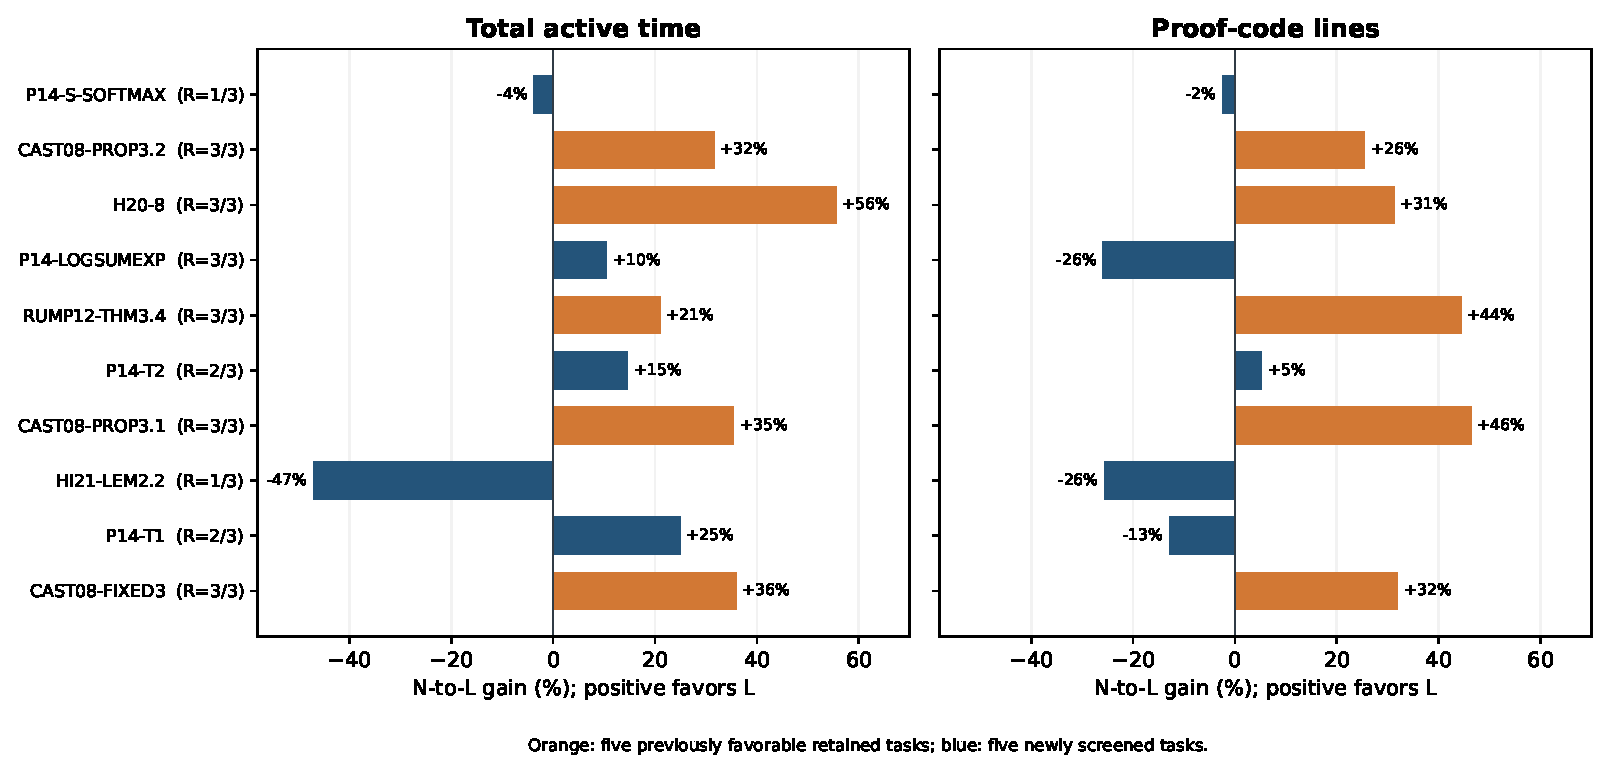
\includegraphics[width=\textwidth]{figures/ten_task_gains.pdf}
\caption{Per-task paired gains. Every task label includes its exact realized
reuse score in parentheses. The chart distinguishes prior favorable tasks
from newly screened tasks rather than pooling them invisibly.\cite{derived}}
\label{fig:tasks}
\end{figure}

\clearpage
\section{Does the selected cohort support the overlap claim?}

The 0--3 score counts \emph{roles} of task-relevant, directly used
NumStability declarations in the final L statement or kernel-checked proof:
foundation, computation interface, and mathematical analysis. It does not
count imports or total declarations and is not an independent measure of
potential library coverage. The annotation is post-outcome. The five
exclusions remove the only score-0 task, one score-2 task, and three score-3
tasks. The retained score counts are 2, 2, and 6 for scores 1, 2, and 3.\src{reuse,derived}

\begin{table}[H]
\centering\small
\begin{tabular}{@{}lrrrr@{}}\toprule
Reuse score & $n$ & Active-time gain (\%) & Proof-line gain (\%) & Token gain (\%)\\\midrule
1/3 & 2 & -9.1 & -4.2 & -41.0 \\
2/3 & 2 & +19.3 & -1.2 & -20.2 \\
3/3 & 6 & +31.1 & +31.4 & -37.3 \\
\bottomrule

\end{tabular}
\caption{Aggregate N-to-L gains within each retained score stratum. Positive
favors L. There is no score-0 task left in this selected set; score-2 proof
lines do not improve. Small, unequal and selected groups preclude a causal
trend claim.\cite{derived}}
\label{tab:scores}
\end{table}

The selected score strata form a monotone sequence in \emph{aggregate active
time}: $-9.1\%$, $+19.3\%$, $+31.1\%$. The proof-line sequence is $-4.2\%$,
$-1.2\%$, $+31.4\%$; hence a substantial code-size reduction appears only in
the highest stratum. This supports the narrower observation that, \emph{in
this outcome-selected subset}, broader realized reuse accompanies better
aggregate time and proof-code outcomes. It does not show that more reuse
caused the gains. Five of the six score-3 tasks are the previously favorable
retained tasks. The only new score-3 task, P14-LOGSUMEXP, is faster but has
26.0\% \emph{more} L proof lines.\src{reuse,derived}

\begin{figure}[H]
\centering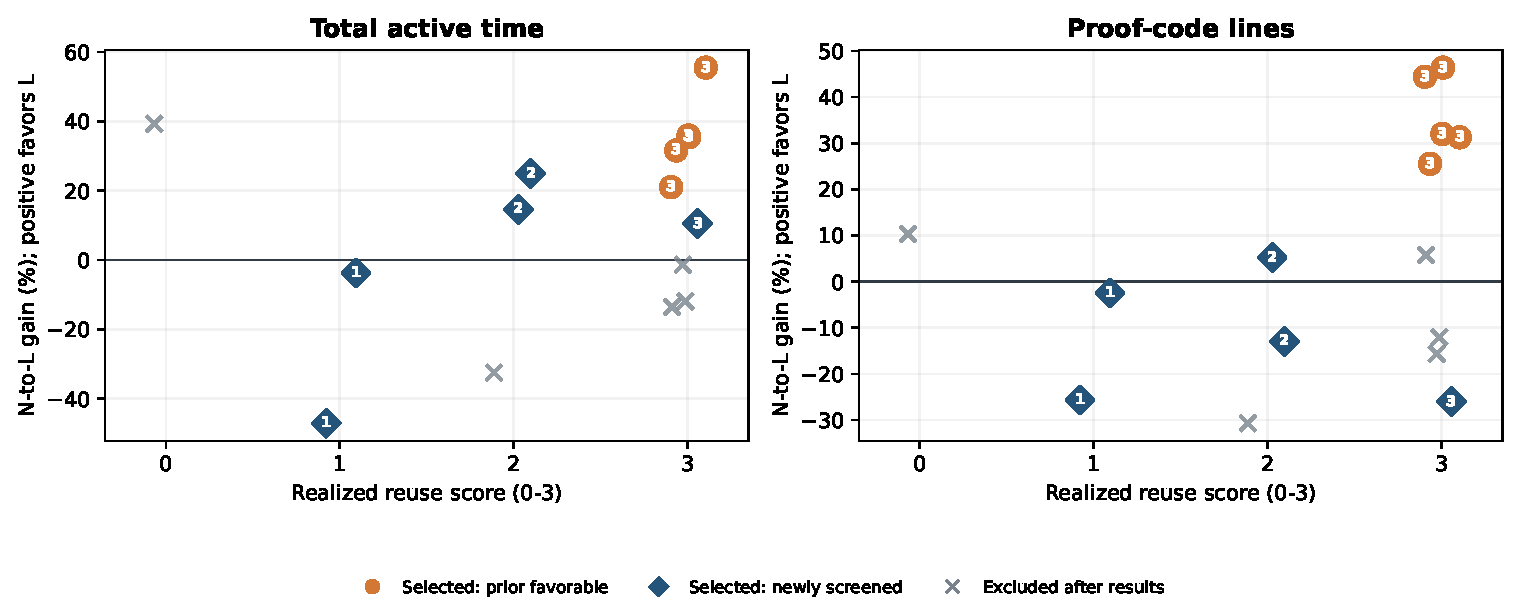
\includegraphics[width=.95\textwidth]{figures/selection_map.pdf}
\caption{All original fifteen pairs remain visible. Grey crosses mark the
five post-hoc exclusions; orange circles and blue diamonds are the ten
included pairs. The numeral inside each included point is its reuse score;
horizontal jitter only separates integer-score ties. These panels expose the
selection behind the apparent score relationship.\cite{metrics,reuse,derived}}
\label{fig:selection}
\end{figure}

\clearpage
\section{Cost decomposition and limits of the claim}

For the ten selected tasks, N and L required 1,389 and 1,490 formalization
seconds, respectively: L was 7.3\% slower before a faithful statement. In
the proof stage, they required 5,590 and 3,920 seconds: L was 29.9\% faster.
The one-time task-neutral L orientation cost another 183 seconds, making
the complete ten-task time sums 6,979 (N) versus 5,593 (L), a 19.9\% L gain.
This is an amortized ten-task sum, not the wall-clock makespan of three
parallel lanes.\src{metrics,primary,derived}

The token picture is unfavorable to L. Formalization used 399,748 N versus
980,733 L net-new tokens; proof used 873,571 N versus 734,899 L. Overall,
the ten pairs used 1,273,319 N versus 1,715,632 L net-new tokens: 34.7\%
\emph{more} for L. Charging the warm scout's 88,468 tokens once raises L
to 1,804,100, or 41.7\% more than N. Task-time search and compilation are
included or excluded according to the frozen controller's contestant clock;
the present filtered tables cannot isolate search as the cause of any one
negative result. Conversation traces would be required to establish such a
mechanism.\src{metrics,primary,derived}

\begin{table}[H]
\centering\small
\begin{tabular}{@{}lrrr@{}}\toprule
Task removed after inspection & Score & Time gain (\%) & Proof-line gain (\%)\\\midrule
\texttt{P14-ALT-SOFTMAX} & 3/3 & -1.4 & -15.7 \\
\texttt{P14-SHIFTED-SUM} & 0/3 & +39.3 & +10.3 \\
\texttt{P14-SHIFTED-LOG} & 3/3 & -13.5 & +5.8 \\
\texttt{P14-SHIFTED-WEIGHTED} & 2/3 & -32.5 & -30.7 \\
\texttt{HI21-EQ2.7} & 3/3 & -11.9 & -12.1 \\
\bottomrule

\end{tabular}
\caption{The removed observations, retained in the source and shown here to
make selection auditable. P14-SHIFTED-SUM was favorable to L despite score
zero, whereas several high-score tasks were unfavorable.\cite{metrics,reuse,derived}}
\end{table}

\paragraph{Defensible conclusion.} In these ten transparently selected,
faithful and fully proved tasks, L reduced total active time and proof-code
size; its largest aggregate gains lie in the highest realized-reuse group.
That demonstrates useful reuse for a slice of numerical-stability problems.
It does \emph{not} establish that lower overlap generally causes loss, that
library expansion alone will fix every negative task, or that the reported
percentages estimate performance on unseen tasks. The full fifteen-task
result remains the primary development evidence. A prospective corpus and
predefined score would be needed for a general coverage-benefit claim.

\section*{Reproduction and sources}
The accompanying README gives the exact three-command rebuild procedure:
verify the primary evidence, run this report's filter script, then compile
the TeX source. The script asserts the original 15 identities, the exact
five exclusions, and the 5+5 selected origin mix. The derived
\path{generated/summary.json} contains the source SHA-256 hashes, selected
IDs, and full-precision aggregates.

\begin{thebibliography}{9}\small
\bibitem{primary} NumStability benchmark, complete fifteen-task evidence
report, \path{paper_bencmark/thesis_report/report.tex} and
\path{output/pdf/report.pdf}, branch
\texttt{codex/numstability-benchmark-thesis-report}, commit
\texttt{30cda8a55}.
\bibitem{metrics} Hash-checked task-level measurements,
\path{paper_bencmark/thesis_report/generated/task_metrics.csv}; primary
verification script \path{paper_bencmark/thesis_report/verify_release.py}.
\bibitem{reuse} Exact-witness realized-reuse rubric and ledger,
\path{paper_bencmark/thesis_report/reuse_obligations.json} and
\path{paper_bencmark/thesis_report/generated/realized_reuse.csv}.
\bibitem{derived} This report's reproducible filter, figures and aggregates,
\path{paper_bencmark/thesis_report/posthoc_10/make_report.py} and
\path{paper_bencmark/thesis_report/posthoc_10/generated/summary.json}.
\end{thebibliography}
\end{document}
